\section*{Цель работы}

\begin{enumerate}
    \item Моделирование и исследование работы ЦАП на основе резистивной
    матрицы R-2R и АЦП прямого действия в LTspice.
\end{enumerate}

\section*{Исследование работы ЦАП}

В соответствии с вариантом разрядность ЦАП 4-бита, ОУ AD746 и $R=10$ кОм.
Соберем схему как на рисунке \ref{fig:r2r_scheme}. С которой получим сигналы
(см. рис. \ref{fig:r2r_signals}). 

\begin{figure}[H]
    \centering
    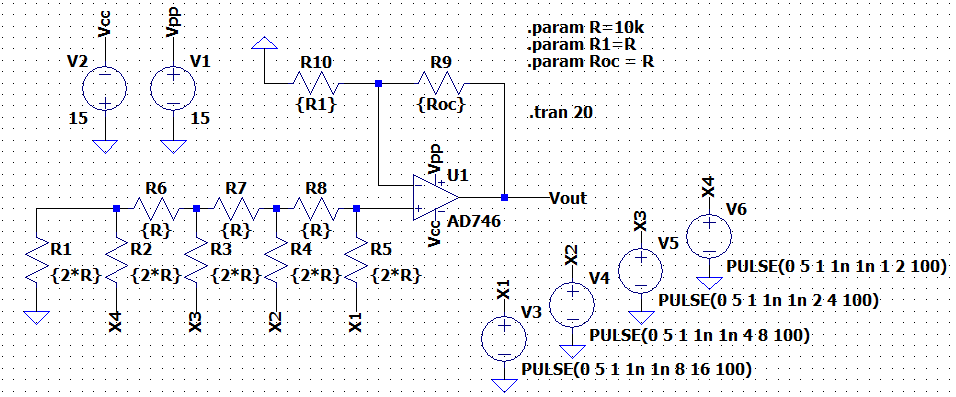
\includegraphics[width=\linewidth]{figs/R-2R_scheme.png}
    \caption{Схема ЦАП R-2R}
    \label{fig:r2r_scheme}
\end{figure}

\begin{figure}[H]
    \centering
    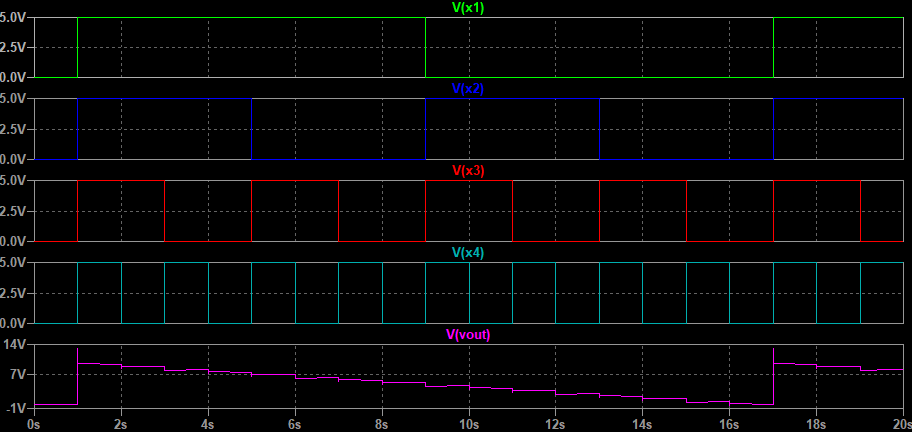
\includegraphics[width=\linewidth]{figs/R-2R_signals.png}
    \caption{Сигналы схемы ЦАП R-2R}
    \label{fig:r2r_signals}
\end{figure}

Из рисунка \ref{fig:r2r_signals} сделаем таблицу \ref{tab:r2r}, в которую
занесем напряжения на входах и выходе. Как можно подметить, выход изменяется линейно.

\begin{table}[H]
    \centering
    \caption{Таблица состояний ЦАП}
    \label{tab:r2r}
    \begin{tabular}{|c|c|c|c|c|}
        \hline
        X1, В & X2, В & X3, В & X4, В & Vout, В \\
        \hline
        5 & 5 & 5 & 5 & 9.37 \\ \hline
        5 & 5 & 5 & 0 & 8.75 \\ \hline
        5 & 5 & 0 & 5 & 8.12 \\ \hline
        5 & 5 & 0 & 0 & 7.50 \\ \hline
        5 & 0 & 5 & 5 & 6.84 \\ \hline
        5 & 0 & 5 & 0 & 6.25 \\ \hline
        5 & 0 & 0 & 5 & 5.62 \\ \hline
        5 & 0 & 0 & 0 & 5.00 \\ \hline
        0 & 5 & 5 & 5 & 4.37 \\ \hline
        0 & 5 & 5 & 0 & 3.75 \\ \hline
        0 & 5 & 0 & 5 & 3.12 \\ \hline
        0 & 5 & 0 & 0 & 2.50 \\ \hline
        0 & 0 & 5 & 5 & 1.87 \\ \hline
        0 & 0 & 5 & 0 & 1.25 \\ \hline
        0 & 0 & 0 & 5 & 0.62 \\ \hline
        0 & 0 & 0 & 0 & 0.00 \\ \hline
    \end{tabular}
\end{table}


\section*{Исследование работы АЦП}

Соберем в LTspice схему как на рисунке \ref{fig:adc_scheme} прямого АЦП с приоритетным 
шифратором, в соответствии с вариантом компаратор LTC1441, $U_{ref}=16$ В.

\begin{figure}[H]
    \centering
    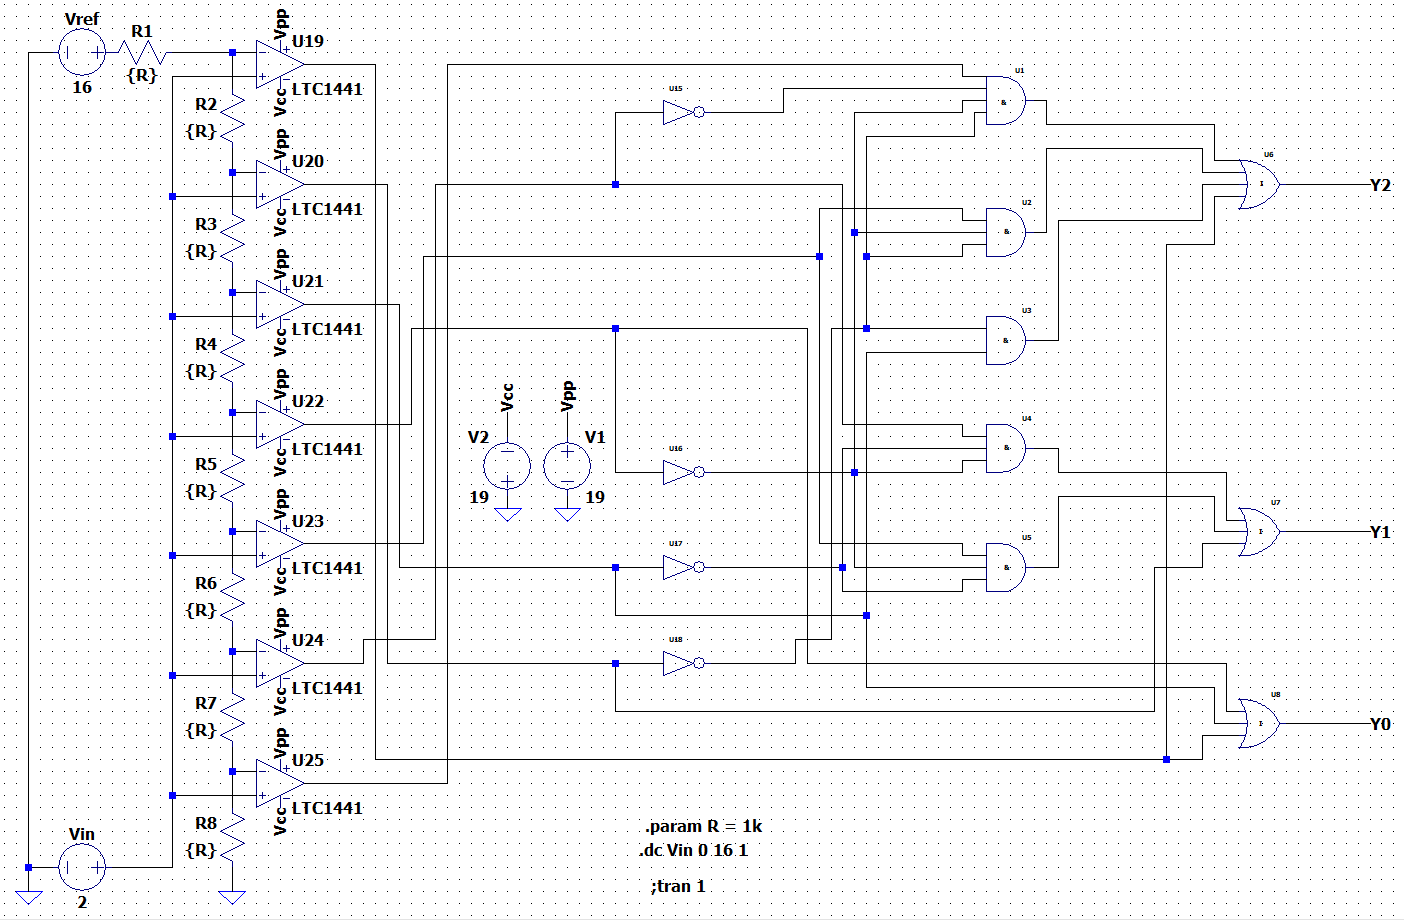
\includegraphics[width=\linewidth]{figs/adc_scheme.png}
    \caption{Схема прямого АЦП с приоритетным шифратором}
    \label{fig:adc_scheme}
\end{figure}

\begin{figure}[H]
    \centering
    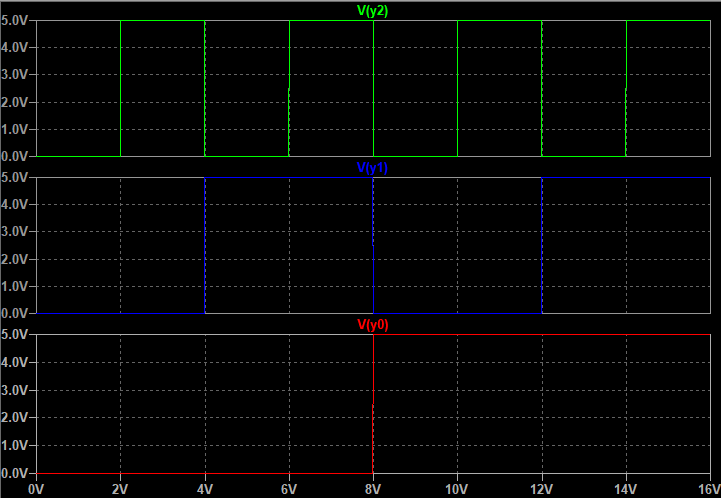
\includegraphics[width=\linewidth]{figs/adc_sig.png}
    \caption{"Шифр" прямого АЦП с приоритетным шифратором при линейно возрастающем
    напряжении на входе}
    \label{fig:adc_signals}
\end{figure}

Шифр прямого АЦП с приоритетным шифратором при линейно возрастающем напряжении на входе
можно увидеть на рисунке \ref{fig:adc_signals}. Из этого составим таблицу состояний
(см. таблицу \ref{tab:adc}). Все работает как и предполагалось.

\begin{table}[H]
    \centering
    \caption{Состояния АЦП}
    \label{tab:adc}
    \begin{tabular}{|c|c|c|c|}
        \hline
        $U_{in}$, В & y0, В & y1, В & y2, В \\ \hline
        <2 & 0 & 0 & 0 \\ \hline
        (2; 4) & 0 & 0 & 5 \\ \hline
        (2; 6) & 0 & 5 & 0 \\ \hline
        (6; 8) & 0 & 5 & 5 \\ \hline
        (8; 10) & 5 & 0 & 0 \\ \hline
        (10; 12) & 5 & 0 & 5 \\ \hline
        (12; 14) & 5 & 5 & 0 \\ \hline
        >14 & 5 & 5 & 5 \\ \hline
    \end{tabular}
\end{table}


\section*{Заключение}

В данной лабораторной работе мы изучили работу ЦАП R-2R и АЦП прямого действия 
с приоритетным шифратором в LTspice. Были получены графики сигналов и
таблицы состояний.